\documentclass[11pt, A4paper,norsk]{article}
\usepackage[utf8]{inputenc}
\usepackage[T1]{fontenc}
\usepackage{babel}
\usepackage{amsmath}
\usepackage{amsfonts}
\usepackage{amsthm}
\usepackage{amssymb}
\usepackage[colorlinks]{hyperref}
\usepackage{listings}
\usepackage{color}
\usepackage{hyperref}
\usepackage{graphicx}
\usepackage{cite}
\usepackage{textcomp}
\usepackage{float}

\definecolor{dkgreen}{rgb}{0,0.6,0}
\definecolor{gray}{rgb}{0.5,0.5,0.5}
\definecolor{daynineyellow}{rgb}{1.0,0.655,0.102}
\definecolor{url}{rgb}{0.1,0.1,0.4}

\lstset{frame=tb,
	language=Python,
	aboveskip=3mm,
	belowskip=3mm,
	showstringspaces=false,
	columns=flexible,
	basicstyle={\small\ttfamily},
	numbers=none,
	numberstyle=\tiny\color{gray},
	keywordstyle=\color{blue},
	commentstyle=\color{daynineyellow},
	stringstyle=\color{dkgreen},
	breaklines=true,
	breakatwhitespace=true,
	tabsize=3
}

\lstset{inputpath="C:/Users/Torstein/Documents/UiO/Fys2130/Python programmer"}
\graphicspath{{C:/Users/Torstein/Documents/UiO/Fys2130/"Python programmer"/}}
\hypersetup{colorlinks, urlcolor=url}

\author{Torstein Solheim Ølberg}
\title{Svar på Oblig nr. 2 i Fys2130}



%\lstinputlisting{Filnavn! type kodefil}
%\includegraphics[width=12.6cm,height=8cm]{Filnavn! type png}



\begin{document}
\maketitle
	\begin{center}
\Large \textbf{Oppgaver}
	\end{center}








	\begin{flushleft}
\textbf{Kapittel 3}
	\end{flushleft}
		\paragraph{3.}
			\subparagraph{1}
			\begin{flushleft}
Utrykket for resonansfrekvensen blir større for større verdi av $\omega_0$ og mindre for større verdi av dempningsfaktoren $b$. Siden begge disse faktorene har samme rolle i utrykket for $Q$-faktoren: $$Q = \frac{m \omega_0}{b}$$ betyr dette at det er enklere å få en større $Q$ hvis resonansfrekvensen også er større.
			\end{flushleft}









		\paragraph{6.}
			\begin{flushleft}
Hvis det ikke er noen dempning på svigningen og systemet som svinger blir utsatt for en harmonisk kraft som har frekvens lik resonansfrekvensen til systemet vårt. Dette fordi Amplituden ikke vil bli mindre på noen måte siden det ikke er noen dempning, og når kraften alltid er i retning av hastigheten til systemet vil amplituden bare vokse og vokse til systemet blir ødelagt eller noe annet skjer som får svigningen til å slutte. \\
Hvis den påtrykte kraften sin frekvens er bitte litt forskjellig fra resonansfrekvensen, vil kraften sakte men sikkert drive ut av synkronisering med svigningene og dermed virke mer og mer dempende.
			\end{flushleft}
\clearpage








	\begin{flushleft}
\textbf{Kapittel 4}
	\end{flushleft}
		\paragraph{1.}
			\begin{flushleft}
Runge Kutta fire er vanligvis en bedre metode enn Eulers metoden fordi den lager fire tilnærminger til stigningstallet til funksjonen istedenfor en slik som Euler gjør.
			\end{flushleft}
			









		\paragraph{2.}
			\begin{flushleft}
De øverste to figurene sier at denne pendelen svinger frem og tilbake med lavere og lavere utslagsvinkel. Svigningen startet med en amplitude på $1.5$ radianer, men i løpet av ca. åtte sekunder ser det ut til at amplituden er nede på $1.25$. I tillegg viser fasediagrammet at pendelen startet med en utgangsvinkelhastighet på seks $\frac{rad}{s}$ og denne vinkelhastigheten sitt maksimautslag avtar også. \\
De to nederste figurene viser at med disse initialbetingelsene vil pendelen foreta en fulstendig rotasjon og deretter fortsette svigningen frem og tilbake. Det er også interessant å få med seg at det ser ut som pendelen svinger helt opp til den står rett opp, etter den første fullstendige rotasjonen, og at den blir stående der litt før den begynner å falle ned igjen og fortsette pendlingen frem og tilbake. Av fasediagrammet kan vi se at pendelen nå starter med en vinkelhastighet på nesten ti, og at hastighetens maksimalutslag avtar slik som før. Denne gangen kan vi derimot også se at det skjer noe rart når pendelen nærmer seg toppen for andre gang. Da ser vi at vinkelhastigheten plutselig avtar linjært istedenfor etter en sinus-model slik som tidligere. Samme skjer tildels også når pendelen nærmer seg toppen for tredje gang, bare i motsatt retning denne gangen. \\
Dersom vi øker utgangsvinkelhastigheten enda mer vil antageligvis pendelen rotere enda flere ganger, og den første av figurene vil ha en mye lengere stigning før den ender opp i en bølge, mens fasediagrammet vil ha flere bølger før sirkelformen.
			\end{flushleft}










	\begin{flushleft}
\textbf{Kapittel 3}
	\end{flushleft}
		\paragraph{12.}
			\begin{gather*}
\text{Bruker definisjonen av $Q$-faktoren.} \\
Q = \frac{f_0}{\Delta f} = \frac{1313 Hz}{9 \cdot 10^3 Hz} = 0.1459
			\end{gather*}









		\paragraph{13.}
			\subparagraph{a)}
				\begin{flushleft}
Hvis hylet skal rekke å avta nok slik at det er mulig å høre et ekko fra en vegg, så er avstanden nødt til å være så lang at lyden bruker lang nok tid til at hylet fra flaggermusen ikke er hørbar lenger. Vi regner dette punktet som når Energien til svigningene er under nivået $\frac{1}{e}$ og det tar tiden
				\end{flushleft}
				\begin{gather*}
\Delta t = \frac{Q}{\omega_0} \\
\omega_0 = 2 \pi \cdot f \\
\Delta t = \frac{Q}{2 \pi \cdot f} \\
\Delta s = v \cdot \Delta t = v \cdot \frac{Q}{2 \pi \cdot f} = 340 m/s \cdot \frac{100}{2 \pi \cdot 40 \cdot 10^3 Hz} = 0.1353 m \\
\Delta s = 340 m/s \cdot \frac{100}{2 \pi \cdot 100 \cdot 10^3 Hz} = 0.0541 m
				\end{gather*}
				\begin{flushleft}
Siden flaggermusen bare trenger å høre det den høyeste av tonene, holder det at avstanden er litt lengre enn $0.0541 m = 5.41 cm$
				\end{flushleft}









			\subparagraph{b)}
				\begin{flushleft}
Hvis flaggermusa bruker lydpuls på $1000 Hz$ blir avstanden
				\end{flushleft}
				\begin{gather*}
\Delta s = 340 m/s \cdot \frac{100}{2 \pi \cdot 1 \cdot 10^3 Hz} = 5.4113 m
				\end{gather*}
				\begin{flushleft}
Ser da at avstanden må være lenger enn $5.4113 m$
				\end{flushleft}








		\paragraph{18.}
			\subparagraph{a)}
				\begin{flushleft}
Skriver opp likningene $(3.1) = (1)$ og $(3.7) = (2)$
				\end{flushleft}
				\begin{gather}
\ddot{z}(t) + \frac{b}{m} \dot{z}(t) + \omega_0^2 z(t) = \frac{F}{m} \cos (\omega_F t) \\
L \frac{d^2 Q}{dt^2} + R \frac{dQ}{dt} + \frac{1}{C} Q = V_0 \cos(\omega_F t) \\
\text{Hvis disse likningene skal tilsvare hverandre så får vi disse likningene også} \nonumber \\
\begin{tabular} { c|c|c|c}
$L = m$ & $R = b$ & $\frac{1}{CL} = \omega_0^2$ & $V_0 = F$
\end{tabular} \\
\cot(\phi) = \frac{\omega_0^2 - \omega_F^2}{\omega_F \frac{b}{m}} \Rightarrow \cot \phi = \frac{\frac{1}{CL} - \omega_F^2}{\omega_F \frac{R}{L}} = \frac{1}{C \omega_F R} - \frac{\omega_F L}{R} \\
A = \frac{\frac{F}{m}}{\sqrt{\left( \omega_0^2 - \omega_F^2 \right)^2 + \left( \frac{b \omega_F}{m} \right)^2}} \Rightarrow A = \frac{V_0}{\sqrt{\left( \frac{1}{C} - L\omega_F^2 \right)^2 + R^2 \omega_F^2}} \\
f_{amp, res} = \frac{1}{2 \pi} \sqrt{\omega_0^2 - \frac{b^2}{2m^2}} \Rightarrow f_{amp, res} = \frac{1}{2 \pi} \sqrt{\frac{1}{CL} - \frac{R^2}{2L^2}} \\
f_{fase, res} = \frac{1}{2 \pi} \omega_0 \Rightarrow f_{fase, res} \frac{1}{2 \pi \sqrt{CL}} \\
Q = \frac{m \omega_0}{b} \Rightarrow Q = \frac{\sqrt{L}}{R\sqrt{C}}
				\end{gather}











			\subparagraph{b)}
				\begin{gather*}
f_{amp, res} = \frac{1}{2 \pi} \sqrt{\frac{1}{CL} - \frac{R^2}{2L^2}} = \frac{1}{2 \pi} \sqrt{\frac{1}{100 nF \cdot 25 \mu H} - \frac{(1.0 ohm)^2}{2 (25 \mu H)^2}} = 100558 Hz \\
f_{fase, res} \frac{1}{2 \pi \sqrt{CL}} = \frac{1}{2 \pi \sqrt{100 nF \cdot 25 \mu H}} = 100658 Hz
				\end{gather*}












			\subparagraph{c)}
				\begin{gather*}
Q = \frac{\sqrt{L}}{R\sqrt{C}} = \frac{\sqrt{25 \mu H}}{1.0 ohm \cdot \sqrt{100 \cdot 10^{-9} F}} = 15.8
				\end{gather*}









			\subparagraph{d)}
				\begin{gather*}
\cot(\phi) = \frac{1}{C \omega_F R} - \frac{\omega_F L}{R} \\
\omega_F = \sqrt{\frac{1}{CL} - \frac{R^2}{2 L^2}} = 631823 Hz \\
\phi = \cot^{-1} (0.03443) \approx \frac{\pi}{2} \cdot k \pi \hspace{2mm}|\hspace{2mm} k = 1,2,3,... \\
\text{Vi må altså avgjøre om det er $\frac{\pi}{2}$ eller $- \frac{\pi}{2}$}
				\end{gather*}
				\begin{flushleft}
For at systemet ikke skal stoppe veldig fort på grunnav at det er i motfase er det nødt til å være i fase, og da blir vinkelen lik $\frac{\pi}{2}$
				\end{flushleft}
\clearpage









	\begin{flushleft}
\textbf{Kapittel 4}
	\end{flushleft}
		\paragraph{4.}
			\subparagraph{a)} \hspace{1mm}

				\begin{figure}[H]
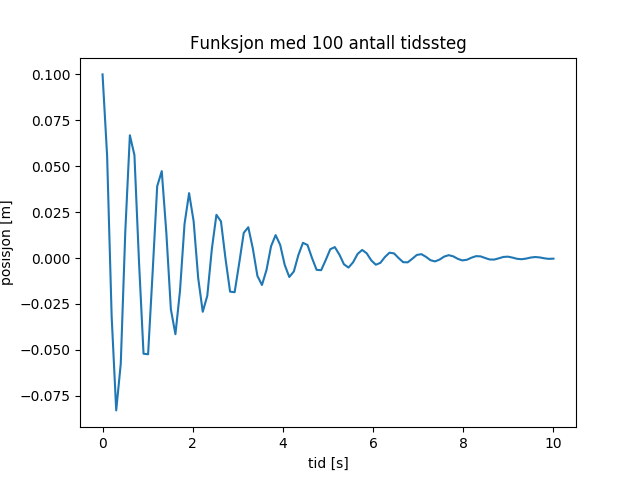
\includegraphics[width=12.6cm,height=8cm]{Figur_0000.png}
				\end{figure}
				\begin{figure}[H]
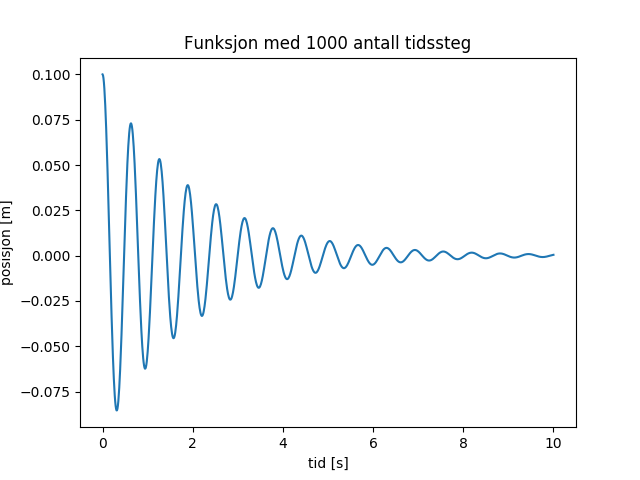
\includegraphics[width=12.6cm,height=8cm]{Figur_0001.png}
				\end{figure}
				\begin{figure}[H]
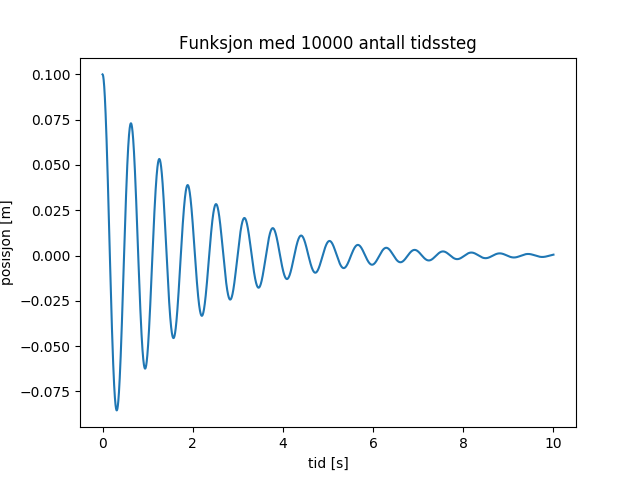
\includegraphics[width=12.6cm,height=8cm]{Figur_0002.png}
				\end{figure}
				\begin{figure}[H]
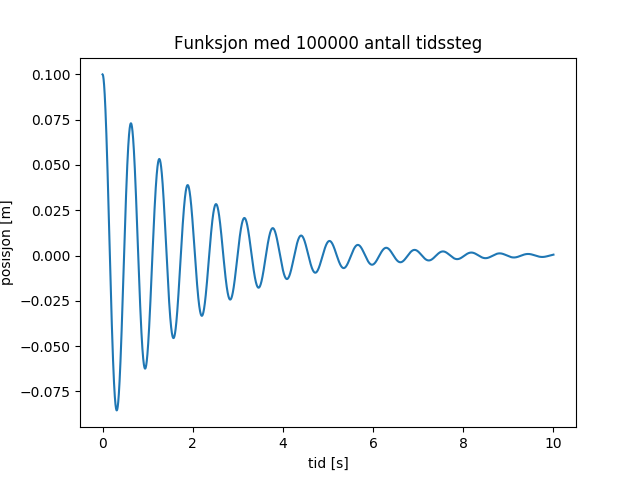
\includegraphics[width=12.6cm,height=8cm]{Figur_0003.png}
				\end{figure}
\lstinputlisting{Oblig2_4_4a.py}
				\begin{gather*}
\ddot{z}(t) = - \frac{b}{m} \dot{z}(t) - \frac{k}{m} z(t) \\
\text{Fra side 14 i kompendiet vet vi at en løsning for denne likningen er} \\
z(t) = e^{- \gamma t} A \cos ( \omega' t + \phi ) \\
\text{der $\gamma = \frac{b}{2m}$, $\omega = \sqrt{\frac{k}{m}}$ og $\omega' = \sqrt{\omega^2 - \gamma^2}$} \\
z(t) = e^{- \frac{b}{2m} t} A \cos \left( \sqrt{\omega^2 - \gamma^2} t +  \right) \\
e^{- \frac{b}{2m} t} A \cos \left( \sqrt{\frac{k}{m} - \left( \frac{b}{2m} \right)^2} t +  \phi \right) = e^{- 0.5 t} A \cos \left( \sqrt{100 - 0.5^2} t + \phi \right) \\
z(t) = A e^{-0.5t} \cos(\sqrt{99.75} t + \phi) \\
z(0) = 0.1 = A e^{0} \cos(\phi) = A \cos(\phi) \\
z'(0) = 0 = - 0.5 A e^{0} \cos(\phi) + A e^{0} \sqrt{99.75} \sin(\phi) = A(\sin(\phi) - \frac{1}{2}\cos(\phi)) \\
\phi = arctan\left( \frac{1}{2} \right) \approx 0.4636 \\
0.1 = A \cos \left( \arctan \left(\frac{1}{2} \right) \right) = A \left( \frac{2}{\sqrt{5}} \right) \\
A = \frac{\sqrt{5}}{2 \cdot 10} = \frac{\sqrt{5}}{20} \approx 0.1118 \\
z(t) = 0.1118 e^{-0.5t} \cos \left( \sqrt{99.75} t + \arctan\left( \frac{1}{2} \right) \right) \\
\text{Fra analytisk likning:} \\
z(\pi) = 0.021166 \\
\text{Fra numerisk løsning:} \\
z(\pi) = 0.020726
\text{Virker som analytisk og numerisk løsning er ganske like.}
				\end{gather*}








			\subparagraph{b)}
				\begin{flushleft}
Jeg valgte parameterne mine sånn fordi det står i kompendiet at det er de jeg skal velge.
				\end{flushleft}
				\begin{figure}[H]
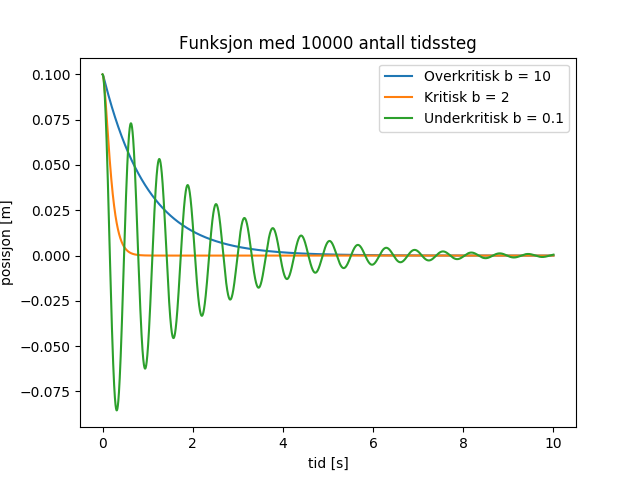
\includegraphics[width=12.6cm,height=8cm]{Figur_0004.png}
				\end{figure}
\lstinputlisting{Oblig2_4_4b.py}








			\subparagraph{c)} \hspace{1mm}
				\begin{figure}[H]
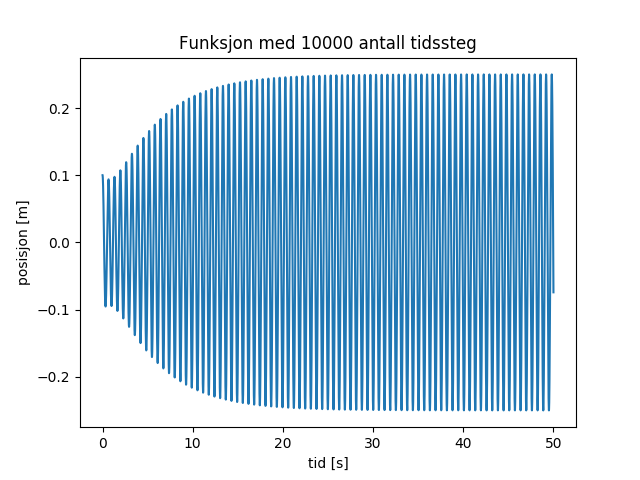
\includegraphics[width=12.6cm,height=8cm]{Figur_0005.png}
				\end{figure}
				\begin{figure}[H]
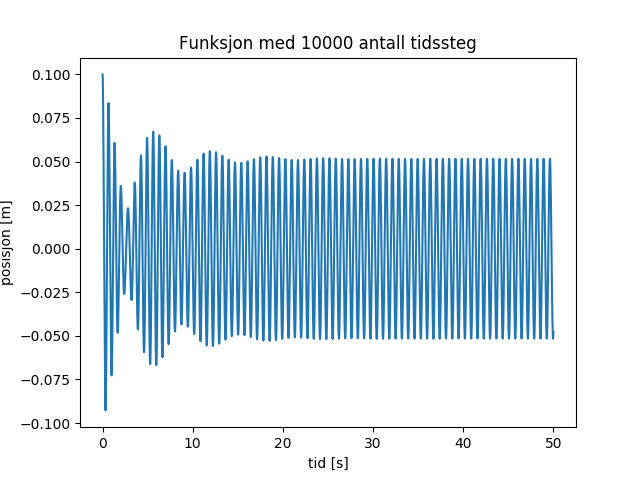
\includegraphics[width=12.6cm,height=8cm]{Figur_0006.png}
				\end{figure}
				\begin{flushleft}
Disse plottene svarer til plottene i figur 3.7 bare at de er med våre variabler og ikke med variablene brukt i figur 3.7.
				\end{flushleft}
\lstinputlisting{Oblig2_4_4c.py}








			\subparagraph{d)} \hspace{1mm}
				\begin{figure}[H]
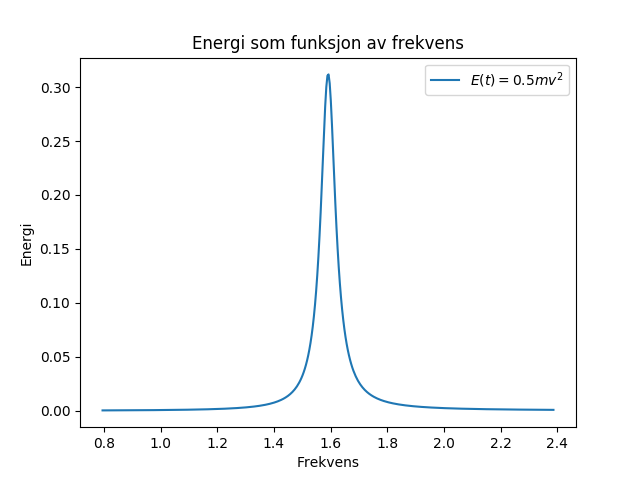
\includegraphics[width=12.6cm,height=8cm]{Figur_0007.png}
				\end{figure}
				\begin{gather*}
Q = \frac{f_0}{\Delta f} = \frac{1.6}{1.62479 - 1.55852} = \frac{1.6}{0.06627} = 24.14 \\
Q = \sqrt{\frac{m k}{b^2}} = \sqrt{\frac{0.1 kg \cdot 10 N/m}{(0.04 kg/s)^2}} = 25.0
				\end{gather*}
				\begin{flushleft}
Det virker som det er fint mulig å lese av Q verdien på grafen. I hvert fall sånn cirka
				\end{flushleft}






		\paragraph{7.}
			\begin{flushleft}
Kan ikke skjønne hvordan denne oppgaven er forskjellig fra deloppgaven rett over, så antageligvis har jeg misforstått enten denne eller den forrige oppgaven.
			\end{flushleft}
\end{document}